% !TEX root = ..\Main.tex
\chapter{Introductory Material}
\label{chapterlabel:Introduction}

%\red{Some stuff about things.\cite{example-citation} Some more things. Inline citation: \bibentry{example-citation}. Motivate the $\ILC~$ model using the paragraph written in the low depth circuit paper. Explain how it enables separation of commitment design, and designing better $\ILC~$ protocols with choices of polynomials, even though the zero-knowledge machinery has not really changed. Separate security proofs into proving properties of specific commitment scheme, proving properties of ILC protocol, and proving security of generic compilation procedure. ===============================================}

\section{Introduction}

A zero-knowledge proof~\cite{GoldwasserMR85} is a protocol between two parties: a prover and a verifier. The prover may want to convince the verifier that an instance $u$ belongs to a specific language $\LL$ in NP. She wants to convince the verifier that the instance $u\in \LL$ is a true statement without revealing any confidential information. Naturally, the protocol should not leak any secret information which is unknown to the verifier and could make the statement easier to prove.

Zero-knowledge proofs are widely used in cryptography since it is often useful to verify that a party is following a protocol without requiring her to divulge secret keys or other private information. Applications range from digital signatures and public-key encryption to secure multi-party computation schemes with strong security guarantees, anonymous credentials, and verifiable cloud computing.

More formally, a zero-knowledge proof consists of a triple of algorithms $(\crsgen,\prover,\verifier)$. These are the prover \prover\ and the verifier \verifier, and they engage in the protocol. The common-reference-string generator \crsgen\ produces the necessary setup information for \prover\ and \verifier\ to run the protocol. In this thesis, the prover and verifier are interactive algorithms. Based on the setup information produced by the generator, the prover and the verifier exchange messages. At the end of the protocol, the verifier decides whether the proof was convincing or not, and accepts or rejects the proof.

Zero-knowledge proofs satisfy three basic requirements.

\paragraph{Completeness.} When the statement is true, the prover always succeeds in convincing the verifier. In other words, when $u \in \LL$, and the prover has a valid witness $w$, the verifier will always accept at the end of the protocol. Completeness can be viewed as more of a functionality requirement than a security requirement, and this property guarantees that the protocol works properly when the prover and verifier are honest.

\paragraph{Soundness.} When the statement is false, or the prover does not know a valid witness, the prover can practically never convince the verifier, and the verifier will almost always reject the proof. Viewed another way, if the verifier accepted the proof, then $u \in \LL$, and the prover has a valid witness $w$. Soundness can be seen as a converse to completeness. It is a security requirement which protects the verifier from being fooled into accepting by a malicious prover. As such, it can be seen as a property of the verification algorithm.

\paragraph{Zero-Knowledge.} Despite taking part in the protocol with the prover, the verifier can never learn anything from the interaction except that the statement is true. This is modelled by showing that the entire interaction between the prover and the verifier can be simulated without any knowledge of the witness. If convincing-looking proofs can be simulated without any secret information, then it follows that nothing secret can be learned from real proofs. Zero-knowledge is a security requirement which protects the prover against a malicious verifier who is trying to learn the prover's secrets. As such, it can be seen as a property of the proving algorithm.

%Given a zero-knowledge proof, how do we evaluate whether or not it is a `good' one? 
%
%\red{Prover and verifier computation}
%\red{Communication}
%\red{Interaction}
%\red{Assumption}
%\red{Pre-processing/setup}
%\red{Public Coin}
%\red{Stronger and Weaker Security Notions, including...}
%\red{Proof-of-knowledge}
%\red{Honest-Verifier Zero-Knowledge}

Many efficient zero-knowledge proofs are based on the discrete logarithm assumption~\cite{Schnorr91,Cramer1998a,Groth2009b,Seo2011a,BootleCCGP16,BunzBBPWM18,GrothK15,BootleCCGGP15,BayerG13,BootleG18}. Although efficiency has improved over time, it looks as though all of these protocols draw on the same small collection of techniques, some used for improbing efficiency, and some for proving security.

For instance, all of the protocols above use commitment schemes. These allow either party to `commit' to a message, so that the message stays hidden but is fixed relative to the commitment, and can be revealed later. A party can commit to a message $m$ by applying a commitment algorithm with $m$ as input, and obtain $c$, a commitment to $m$. The commitment $c$ can then be sent to other parties. Later, the party can `open' $c$ by revealing $m$. The other parties may then check that $c$ corresponds to $m$.

Commitment schemes satisfy two basic requirements.

\paragraph{Hiding.} Like a sealed envelope, a commitment should hide the message inside. The commitment $c$ should not leak any information about $m$.

\paragraph{Binding.} Once an envelope is sealed, it is not possible to change the message inside without breaking open the envelope. Given a commitment $c$ to a message $m$, it should be impossible to open $c$ to a different message.

The protocols all use homomorphic commitments, where one can combine two commitments together to obtain a commitment to the sum of the messages.

These protocols also follow a similar pattern of interaction between the prover and the verifier. The prover sends an initial message $a_1$ to the verifier. The verifier responds with a random challenge value $e_1$. The prover sends another message $a_2$ to the verifier, who responds with another random challenge $e_2$. This process continues for $n$ rounds, until messages $a_n$ and $e_n$ have been exchanged. The prover sends a final message $a_{n+1}$ to the verifier, and then the verifier decides whether to accept or reject.

In fact, there are even more similarities to be observed. For many protocols, the prover's messages $a_1$, $a_2$ up to $a_n$ are actually single or possibly multiple commitments to secret values obtained by the prover, computed using the witness or the random challenge values that the prover has seen up to that point. The prover's final message $a_{n+1}$ is often a specially chosen sum or linear combination of the secret values that the prover committed to earlier. Then, the verification algorithm involves checking that $a_{n+1}$ really is the correct sum or linear combination of the prover's secret values, using the commitments to achieve this.

In their security proofs, the protocols all seem to use the same techniques, based on polynomial algebra, polynomial identity testing and linear algebra. In fact, on the whole, it does not seem important that the protocols are based on the discrete logarithm assumption, just that they use homomorphic commitment schemes to commit to the elements of finite fields.

One can ask whether it is possible to find the techniques common to all interactive zero-knowledge protocols based on the discrete logarithm assumption, and place them into a single framework. This would drastically simplify the tasks of designing protocols, and proving mathematically that they are secure. Having fully understood or implemented one protocol of this type, it would be much easier to understand or implement any other. In this thesis, we will explore the question of whether there is an information-theoretic framework which provides a good abstraction for discrete-logarithm based interactive zero-knowledge protocols.

However, the framework is useless unless it can be used to create efficient protocols for a wide range of tasks. Thus, we can extend our question in several directions, and propose the following hypothesis for investigation.

There is an information-theoretic framework which provides a good abstraction for discrete-logarithm based interactive zero-knowledge protocols, and further;
\begin{enumerate}
\item The efficiency of information-theoretic protocols in the framework accurately models the efficiency of real protocols.
\item There are efficient protocols in the framework for many different languages.
\item The framework is useful for designing protocols outside the discrete-logarithm setting.
\end{enumerate}

\section{Contributions}

As a building block in our arguments, we present an adaptation of the polynomial commitment sub-protocol appearing in \cite{BootleG18}, which allows the prover to commit to a polynomial so that the verifier can learn an evaluation of the polynomial in a secure manner. The sub-protocol has square-root communication complexity in the degree of the polynomial.

\paragraph{Zero-Knowledge Proofs for Low-Depth Circuits} While very efficient, arguments for general statements, like arithmetic circuit satisfiability, often make use of generic reductions and complex machinery, and fail to be as efficient as arguments specialised for a particular language. We give a zero-knowledge proof for low-depth circuits. In doing so, we bridge the gap between general and simple languages in three ways.

Firstly, we provide a framework to describe the types of languages commonly encountered. Protocols such as the $1$-out-of-$N$ membership argument of  \cite{GrothK15}, and the polynomial evaluation argument of \cite{BayerG13} prove membership in languages where the witnesses are zeroes of low-degree polynomial relations. In other words, the statement is an arithmetic circuit of low degree, and part of the witness is a satisfying assignment for the circuit. We give a general relation which allows us to recover specific protocols by instantiating with concrete polynomial relations. By separating the task of developing more efficient ways to perform the zero knowledge proof, and the task of designing better relations to describe a given language, we can explain the logic behind past optimisations of membership proofs in \cite{GrothK15,BootleG18}, and produce new optimisations for membership proofs and polynomial evaluation proofs.

Secondly, we unify the approaches used in \cite{GrothK15,BayerG13,BootleCCGGP15} to construct zero-knowledge proofs for membership and polynomial evaluation, which can all be viewed as employing the same construction method. The constructions of zero-knowledge arguments for low degree polynomial relations in these works proceed by masking an input variable $u$ as $f_u = ux+u_b$, using a random challenge $x$ and a random blinder $u_b$. During the proof, the polynomial or circuit from the statement is computed with $f_u$ in place of $u$, so that the original relation appears in the leading $x$ coefficient. The communication and computational complexity of the resulting arguments is determined by the degree of the polynomial relation and the number of inputs. By contrast, the complexity of general arithmetic circuit protocols is determined by the number of gates. In the case of \cite{BootleG18}, the authors embed a polynomial evaluation argument for a polynomial of degree $N$ into a low degree polynomial with $\log N$ inputs and degree $\log N$, obtaining a protocol with $O(\log N)$ communication using $3$ moves, and requiring $O(\log N)$ operations to form cryptographic commitments. On the other hand, a polynomial of degree $N$ requires $N$ multiplication gates to evaluate in general, so the best arithmetic circuit protocol \cite{BunzBBPWM18} can only achieve $O(\log N)$ communication in $O(\log N)$ moves, and uses $O(N)$ operations to form cryptographic commitments. In particular, in some settings, like the discrete logarithm setting, forming cryptographic commitments is based on computing exponentiations in a group of prime order. The cost of computing exponentiations is usually much higher than that of computing finite-field multiplications. Computing $O(\log N)$ group exponentiations rather than $O(N)$ leads to a significant performance advantage when considering implementation on constrained devices.

Bayer \cite{Bayer2014} gives two efficient batch proofs for multiplication and polynomial evaluation, which achieve a square-root communication overhead in the number of proofs to be batched. The key to achieving square-root overhead in \cite{Bayer2014} is to use Lagrange interpolation to embed many instances of the same relation into a single field element. This technique can be applied more generally to produce efficient batch proofs for the low-degree relations described above. Furthermore, by combining this with the polynomial commitment subprotocol in section \ref{subsec:polycommit}, we improve the communication cost of the batched proof from $\sqrt{t}c$ to $\sqrt{tc}$, where $c$ is the communication cost of the original non-batched proof, and $t$ is a large number representing the number of proofs to be batched together. 

Thirdly, we exhibit a general protocol in our framework and show how to recover protocols of previous works with some optimisation. More specifically, we give new $1$-out-of-$N$ membership arguments and  polynomial evaluation arguments. Our new instantiations simultaneously decrease communication costs and reduce prover and verifier computation, while retaining the conceptual clarity and simple 3-move structure of the originals. As an example, we obtain the most communication efficient $\Sigma$-protocols for membership or non-membership of a committed value in a public list, in the discrete logarithm setting. We also include an argument for range proofs. Our argument captures the folklore method for performing range proofs, where the prover commits to an integer and the bits of the integer and then proves in zero-knowledge that each committed bit is indeed a bit, and that the bit decomposition corresponds to the integer. This demonstrates the expressivity of our general relation. Incorporating the batching ideas already mentioned, this gives an efficient batch protocol for proving and verifying $t$ instances of the same relation simultaneously.

One notable place where we improve communication efficiency over previous proofs is in our membership and polynomial evaluation proofs instantiated in the discrete logarithm setting, which use a constant number of group elements, but have better communication efficiency regardless of whether the proofs are instantiated in elliptic curve groups or multiplicative subgroups of finite fields. Another is the polynomial evaluation argument which communicates $O(\frac{\log N}{\log \log N})$ commitments and field elements, which is an asymptotic improvement over the previous state-of-the-art, $O(\log N)$ commitments and field elements. Finally, our batch polynomial evaluation argument improves on \cite{Bayer2014} as the cost is proportional to $\sqrt{\log N}$ rather than $\log N$.

See Tables \ref{taEfficiency8} and \ref{taEfficiency9} for our results in the discrete logarithm setting. $N$ is the instance-size, $t$ is the number of batched instances, $\Gr$ means the number of group elements transmitted, $\Z_p$ means the number of field elements transmitted, $(\Gr,exp)$ means the number of group exponentiations and $(\Z_p,\times)$ means the number of field multiplications. In the membership proofs, $N$ is the number of items in the list for which we prove membership. In the polynomial evaluation proofs, $N$ is the degree of the polynomial. In the range proofs, $N$ is the width of the range that we consider.

See Table \ref{taEfficiency1} for our results based on hash-functions.

\footnotetext[1]{We compare against the efficiency when \cite{GrothK15} is instantiated using Pedersen commitments, and the prover and verifier know the openings of the list of commitments.}
\footnotetext[2]{We compare against the efficiency when \cite{BootleCCGGP15} is instantiated using Pedersen commitments rather than Elgamal ciphertexts.}

\afterpage{
\clearpage
\thispagestyle{empty}
\begin{landscape}
\centering
\begin{tabular}{| l | c | c | c | c | c | c | c |}
\hline
Protocol & Reference & \multicolumn{2}{c|}{Communication} & \multicolumn{2}{c|}{Prover Computation}& \multicolumn{2}{c|}{Verifier Computation}\\
&& Hashes & $ \Z_p$ & Hashes & $ (\Z_p,\times)$ & Hashes & $ (\Z_p,\times)$\\
\hhline{|=|=|=|=|=|=|=|=|}
&&&&&&&\\[-1em]
Membership Proof &This Work, \ref{app:member} &  $O( \log N)$ & $O(\log N)$ & $O(\log N)$ & $O(N\log N)$ & $O(\lambda)$ & $O(N)$ \\
%3ary version
\hhline{|=|=|=|=|=|=|=|=|}
&&&&&&&\\[-1em]
Batch Membership Proof &This Work, \ref{app:member} & $O(\sqrt{t \log N})$ & $O(\sqrt{t \log N})$ & $O(t \log tN)$ & $O(tN\log tN)$ & $O(\lambda)$ & $O(tN)$ \\
\hline
&&&&&&&\\[-1em]
Polynomial Evaluation &This Work, \ref{app:poly} & $O(\frac{\log N}{\log \log N})$ & $O(\frac{\log N}{\log \log N})$ & $O(\frac{\log N}{\log \log N})$ & $O(N\log N)$ & $O(\lambda)$ & $O(N)$\\
%n = log2(N)/log2log2(N)
\hhline{|=|=|=|=|=|=|=|=|}
&&&&&&&\\[-1em]
Batch Polynomial Evaluation &This Work, \ref{app:poly} & $O(\sqrt{t \log N})$ & $O(\sqrt{t \log N})$ & $O(t \log tN)$ & $O(tN\log tN)$ & $O(\lambda)$ & $O(tN)$ \\
%6ary version
\hhline{|=|=|=|=|=|=|=|=|}
&&&&&&&\\[-1em]
Range Proof &This Work, \ref{app:range} & $O(\frac{\log N}{\log \log N})$ & $O(\frac{\log N}{\log \log N})$ & $O(\log N)$ & $O(\log N)$ & $O(\lambda)$ & $O(\log N)$\\
%n = log2(N)/log2log2(N)
\hline
&&&&&&&\\[-1em]
Batch Range Proof &This Work, \ref{app:range} & $O(\sqrt{t\log N})$ & $O(\sqrt{t\log N})$ & $O(t \log N)$ & $O(t \log N)$ & $O(\lambda)$ & $O(t\log N)$\\
%6ary version
\hline
\end{tabular}
\captionof{table}{Efficiency comparisons when our low-depth circuit protocol is instantiated with hash functions. Here $N$ is the number of items in the list for a membership proof, or the degree of the polynomial for a polynomial evaluation proof, or the width of the range in a range proof. Then $t$ indicates the number of statements proved at the same time in a batch proof.}\label{taEfficiency1}
\end{landscape}
\clearpage
}

\afterpage{
\clearpage
\thispagestyle{empty}
\begin{landscape}
\centering
\begin{tabular}{| l | c | c | c | c | c | c | c |}
\hline
Protocol & Reference & \multicolumn{2}{c|}{Communication} & \multicolumn{2}{c|}{Prover Computation}& \multicolumn{2}{c|}{Verifier Computation}\\
&& $\Gr $ & $ \Z_p$ & $(\Gr,exp) $ & $ (\Z_p,\times)$ & $(\Gr,exp) $ & $ (\Z_p,\times)$\\
\hhline{|=|=|=|=|=|=|=|=|}
&&&&&&&\\[-1em]
Membership Proof &\cite{BootleCCGP16} & $4 \log N + 8$ & $2\log N + 7$ & $12N$ & $O(N)$ & $4N$ & $O(N)$ \\
\hline
&&&&&&&\\[-1em]
Membership Proof \footnotemark[1] &\cite{GrothK15} & $4 \log N$ & $3 \log N + 1$ & $O(\log N)$ & $O(N \log N)$ & $O(\log N)$ & $O(N)$ \\
\hline
&&&&&&&\\[-1em]
Membership Proof \footnotemark[2] &\cite{BootleCCGGP15} & $\log N + 12$ & $\frac{3}{2} \log N + 6$ & $O(\log N)$ & $O(N \log N)$ & $O(\log N)$ & $O(N)$ \\
\hline
&&&&&&&\\[-1em]
Membership Proof &This Work, \ref{app:member} & $7$ & $4 \log N + 4$ & $O(\frac{\log N}{\log \log N})$ & $O(N\log N)$ & $O(\frac{\log N}{\log \log N})$ & $O(N)$ \\
%binary tree version is better in this case
\hline
&&&&&&&\\[-1em]
Membership Proof &This Work, \ref{app:member} & $2.7\sqrt{\log N}$ & $1.9 \log N+$ & $O(\frac{\log N}{\log \log N})$ & $O(N\log N)$ & $O(\frac{\log N}{\log \log N})$ & $O(N)$ \\
&&&&&&&\\[-1em]
&&$+5$ &$2.7\sqrt{\log N} + 4$ &&&& \\
%3ary version
\hhline{|=|=|=|=|=|=|=|=|}
&&&&&&&\\[-1em]
Batch Membership Proof &This Work, \ref{app:member} & $4.1 \sqrt{t \log N}$ & $4.1\sqrt{t \log N}$ & $O(t \log tN)$ & $O(tN\log tN)$ & $O(\sqrt{t}\log tN)$ & $O(tN)$ \\
\hline
\end{tabular}
\captionof{table}{Efficiency comparisons when our low-depth circuit protocol is instantiated in the discrete logarithm setting. Here $N$ is the number of items in the list for a membership proof. Then $t$ indicates the number of statements proved at the same time in a batch proof.}\label{taEfficiency8}
\end{landscape}
\clearpage
}

\afterpage{
\clearpage
\thispagestyle{empty}
\begin{landscape}
\centering
\begin{tabular}{| l | c | c | c | c | c | c | c |}
\hline
Protocol & Reference & \multicolumn{2}{c|}{Communication} & \multicolumn{2}{c|}{Prover Computation}& \multicolumn{2}{c|}{Verifier Computation}\\
&& $\Gr $ & $ \Z_p$ & $(\Gr,exp) $ & $ (\Z_p,\times)$ & $(\Gr,exp) $ & $ (\Z_p,\times)$\\
\hhline{|=|=|=|=|=|=|=|=|}
&&&&&&&\\[-1em]
Polynomial Evaluation &\cite{BootleCCGP16} & $4 \log N + 8$ & $2\log N + 7$ & $12N$ & $O(N)$ & $4N$ & $O(N)$ \\
\hline
&&&&&&&\\[-1em]
Polynomial Evaluation &\cite{BayerG13}& $4\log N + 2$ & $3\log N + 3$ & $O(\log N)$ & $O(N\log N)$ & $O(\log N)$ & $O(N)$\\
\hline
&&&&&&&\\[-1em]
Polynomial Evaluation &This Work, \ref{app:poly} & $7$ & $3 \log N + 4$ & $O(\frac{\log N}{\log \log N})$ & $O(N\log N)$ & $O(\frac{\log N}{\log \log N})$ & $O(N)$\\
%4ary version
\hline
&&&&&&&\\[-1em]
Polynomial Evaluation &This Work, \ref{app:poly} & $O(\frac{\log N}{\log \log N})$ & $O(\frac{\log N}{\log \log N})$ & $O(\frac{\log N}{\log \log N})$ & $O(N\log N)$ & $O(\frac{\log N}{\log \log N})$ & $O(N)$\\
%n = log2(N)/log2log2(N)
\hhline{|=|=|=|=|=|=|=|=|}
&&&&&&&\\[-1em]
Batch Polynomial Evaluation &\cite{Bayer2014} & $O(\sqrt{t} \log N)$ & $O(\sqrt{t} \log N)$ & $O(t\log N)$ & $O(t N \log N)$ & $O(\sqrt{t}\log N)$ & $O(tN)$ \\
\hline
&&&&&&&\\[-1em]
Batch Polynomial Evaluation &This Work, \ref{app:poly} & $2.8\sqrt{t \log N}$ & $2.8\sqrt{t \log N}$ & $O(t \log tN)$ & $O(tN\log tN)$ & $O(\sqrt{t}\log tN)$ & $O(tN)$ \\
%6ary version
\hhline{|=|=|=|=|=|=|=|=|}
&&&&&&&\\[-1em]
Range Proof &This Work, \ref{app:range} & $7$ & $3\log N + 4$ & $O(\log N)$ & $O(\log N)$ & $O(\log N)$ & $O(\log N)$\\
%4ary version
\hline
&&&&&&&\\[-1em]
Range Proof &This Work, \ref{app:range} & $O(\frac{\log N}{\log \log N})$ & $O(\frac{\log N}{\log \log N})$ & $O(\log N)$ & $O(\log N)$ & $O(\log N)$ & $O(\log N)$\\
%n = log2(N)/log2log2(N)
\hline
&&&&&&&\\[-1em]
Batch Range Proof &This Work, \ref{app:range} & $2.8\sqrt{t\log N}$ & $2.8\sqrt{t\log N}$ & $O(t \log N)$ & $O(t \log N)$ & $O(t \log N)$ & $O(t\log N)$\\
%6ary version
\hline
\end{tabular}
\captionof{table}{Efficiency comparisons when our low-depth circuit protocol is instantiated in the discrete logarithm setting. Here $N$ is the degree of the polynomial for a polynomial evaluation proof, or the width of the range in a range proof. Then $t$ indicates the number of statements proved at the same time in a batch proof.}\label{taEfficiency9}
\end{landscape}
\clearpage
}

\paragraph{Zero-Knowledge Proofs for Arithmetic Circuits.} An arithmetic circuit is a circuit that consists of addition and multiplication gates over a finite field $\F$, whose wires take values from the field. Arithmetic circuits are an attractive target for zero-knowledge protocol design, where the goal is to build an efficient argument system to prove that an arithmetic circuit is satisfiable, meaning that there exist a set of input values to the circuit that produce the specified output value when the circuit is evaluated. The statement is the arithmetic circuit and some specified values for the circuit outputs. The prover's witness is a collection of input values for the arithmetic circuit which give the correct output. There are several reasons why this is useful.
\begin{itemize}
\item Given an arithmetic circuit and outputs, the problem of deciding whether there exist input wire values satisfying the circuit is NP-Complete. Therefore, if we can design zero-knowledge proofs for arithmetic circuit satisfiability, then this implies that we can give zero-knowledge proofs for all NP languages.
\item Many cryptographic systems can be expressed in terms of arithmetic over finite fields of prime order. Given a zero-knowledge proof system for arithmetic circuit satisfiability, we can give zero-knowledge proofs which reason about other cryptographic schemes, often in order to provide stronger security guarantees.
\item There exist compilers which take computer programs written in C \cite{PHGR13,WahbySRBW15} (avoiding certain commands) and convert them into arithmetic circuits. Then, a zero-knowledge proof for arithmetic circuit satisfiability can become a zero-knowledge proof that the C program was executed correctly.
\end{itemize}

We provide two honest verifier zero-knowledge arguments for arithmetic circuit satisfiability. Results for discrete-logarithm arguments are given in Table \ref{table:previous} and results for hash-based arguments in Table \ref{table:previous2}.

In general, the arguments have a square-root communication complexity. The arguments work by reducing the problem of verifying arithmetic circuit satisfiability to the problem of checking that the prover knows that for three commitments, two correspond to committed vectors of values, and the third contains the scalar product of the two vectors. 

\paragraph{3-Move Protocol for Arithmetic Circuit Satisfiability}

We give a 3-move protocol for arithmetic circuit satisfiability. The argument has sublinear communication costs and fewer rounds of interaction than any previously published arguments with sublinear communication in the discrete logarithm setting, and highlights some interesting subtleties in our communication model. When instantiated using Pedersen commitments, this gives the first arithmetic circuit satisfiability protocol with a square-root communication complexity in only three moves. Unfortunately, the argument has a large (superlinear) computational cost for both the prover and the verifier, so is presented mostly for theoretical interest.

%The second argument has better practical efficiency, and when instantiated using a commitment scheme with a few special properties, a special protocol for scalar products leads to an argument that only requires {\em logarithmic} communication complexity.

We start from the circuit satisfiability argument of Groth~\cite{Groth2009b}, which requires 7 moves and has square root communication complexity in the \emph{total} number of gates. In this argument the prover commits to all the wires using homomorphic multicommitments, verifies addition gates using the homomorphic properties, and uses a product argument to show that the multiplication gates are satisfied.

We first improve Groth's argument into a 5-move argument with square root communication complexity in the number of \emph{multiplication gates} only.
%
We achieve fewer moves compared to~\cite{Groth2009b} by avoiding generic reductions to linear algebra statements.
%
We remove the communication cost of the addition gates in the argument by providing a technique that can directly handle a set of Hadamard products and linear relations together.

\begin{table}
%\hspace{-20mm}
\centering
\begin{tabular}{|c|c|ccc|cc|cc|}
\hline
Reference & Moves &\multicolumn{3}{c|}{ Communication}&\multicolumn{2}{c|}{Prover Complexity}&\multicolumn{2}{c|}{Verifier Complexity}\\
&& $\Gr$ &\;\;& $\Z_p$ & exp. & mult. & exp. & mult. \\
\hline
\cite{Cramer1998a}& 3& $6N$  && $5N +2$ & $6N $ & $6N$& $6N$ & $0$ \\%\cite{CD97}& 3& $6N$  & $5N +2$ & $6N+\frac{A}{2\sep} $ & $6N$& $6N+\frac{A}{2\sep} $ & $0$ \\
\cite{Groth2009b}& 7 &$9 \sqrt{N}+4$&&$7\sqrt{N}+6$&$\frac{6N}{\log{N}}$ &$O\left(N \log N\right)$&$\frac{39\sqrt{N}}{\log{N}}$&$O\left(N\right)$ \\
\cite{Groth2009b}& $O(\log{N})$ &$2\sqrt{N}$&&$7\sqrt{N}$&$\frac{6N}{\log{N}}$ & $O(N)$ &  $\frac{18\sqrt{N}}{\log{N}}$&$O\left(N\right)$\\
\cite{Seo2011a}&5&$30\sqrt{N}$ &&$7\sqrt{N}$&$\frac{6N}{\log{N}}$  &$O\left(N\log N\right)$& $\frac{77\sqrt{N}}{\log{N}}$&$O\left(N\right)$\\
\cite{BunzBBPWM18} & $O(\log{N})$  %\red{when m=2, mu = log N - 1}
& $2\log{N}$ &&$O(1)$& $ O(N)$  & $O(N)$ & $O(N)$&$O(N)$ \\
\hline
This work & 3& $O(\sqrt{N})$&&$O(\sqrt{N})$&$O(\frac{N^{3/2}}{\log{N}})$& $O(N^2)$ &$\frac{N}{\log N}$ & $O(N^{3/2})$ \\
\hline
This work & 5& $2\sqrt{N}$&&$2\sqrt{N}$&$\frac{6N}{\log{N}}$& $3N \log{N}$ &$\frac{8\sqrt{3N}}{\log{N}}$ & $O(N)$ \\
\hline
This work & $O(\log{N})$  %\red{when m=2, mu = log N - 1}
& $4\log{N}$ &&$2\log{N}$& $ 12N$  & $O(N)$ & $4N$&$O(N)$ \\
\hline
\end{tabular}
\vspace{.2cm}
\caption{Efficiency comparison between our 5-move argument in the discrete logarithm setting and the most efficient constant-move interactive zero-knowledge arguments relying on discrete logarithms and hash-functions. We express communication in terms of numbers of group elements $\Gr$ and field elements $\Z_p$. We express computational costs in terms of numbers of exponentiations over $\Gr$ and multiplications over $\Z_p$. The efficiency displayed is for a circuit with $N$ multiplication gates.\label{table:previous}} 
\end{table}

\begin{table}
\vspace{20mm}
\centering
\begin{tabular}{|c|c|cc|cc|cc|}
\hline
Reference & Moves &\multicolumn{2}{c|}{ Communication}&\multicolumn{2}{c|}{Prover Complexity}&\multicolumn{2}{c|}{Verifier Complexity}\\
&& Hashes & $\Z_p$ & Hashes & mult. & Hashes & mult. \\
\hline
\cite{CCS:AHIV17}& $O(1)$& $O(\sqrt{N})$  & $O(\sqrt{N})$ & $O(\sqrt{N})$ & $O(N\log N)$& $O(\sqrt{N})$ & $O(\sqrt{N})$ \\
\cite{BootleCGGHJ17}& $O(\log \log N)$ &$O(\sqrt{N})$&$O(\sqrt{N})$&$O(\sqrt{N})$ &$O\left(N \log N\right)$&$O(\lambda)$&$o(N)$ \\
\cite{Ben-SassonBHR18}& $O(1)$ &$O(N)$&$O(N \log N)$&$O(N)$ & $O(N \log N)$ &  $O(\log N)$&$O(\log N)$\\
\hline
This work & 3& $O(\sqrt{N})$&$O(\sqrt{N})$&$O(\frac{N^{3/2}}{\log{N}})$& $O(N^2)$ &$O(\lambda)$ & $O(N^{3/2})$ \\
\hline
This work & 5& $O(\sqrt{N})$&$O(\sqrt{N})$&$O(\sqrt{N})$& $O(N \log{N})$ &$O(\lambda)$ & $O(N)$ \\
\hline
\end{tabular}
\vspace{.2cm}
\caption{Efficiency of our hash-based arguments for arithmetic circuits. The efficiency displayed is for a circuit with $N$ multiplication gates.\label{table:previous2}} 
\vspace{-.5cm}
\end{table}

\paragraph{Logarithmic Complexity Argument.}
In spite of all these improvements, the above argument still requires square root communication complexity with respect to multiplication gates. In the first move the prover commits to all circuit wires using $3m$ commitments to $n$ elements each, where $mn=N$ is a bound on the number of multiplication gates, and in the last move after receiving a challenge he opens commitments that can be constructed from the previous ones and the challenge. The communication complexity is $O(m+n)$. This is minimised when $m, n = O(\sqrt{N})$, which gives square-root communication complexity.

Our key idea to break this square root communication complexity barrier is to replace the last opening step in this protocol with a special protocol for scalar products. In Section~\ref{se:innerproduct} we provide an argument system for this problem, which only requires a logarithmic communication with respect to the vector sizes. The argument is built in a recursive way, reducing the size and complexity of the statement further in each recursion step. This uses a special property of commitments, namely homomorphic properties with respect to the keys. Pedersen commitments, based on the discrete logarithm assumption, satisfy this property. As a result, using this inner product argument as a subroutine in our main argument, and instantiating with Pedersen commitments, we obtain an arithmetic circuit satisfiability argument with logarithmic communication complexity based on the discrete logarithm assumption. This argument was the first of its kind. The constants in the complexities of the protocol have since been improved in \cite{BunzBBPWM18}.

When using a logarithmic number of moves and applying a reduction similar to~\cite{BG12}, our scheme dramatically improves the communication costs with respect to all previous work without incurring any significant overhead. We note that~\cite{BG12} uses a similar reduction to reduce computation whereas we use it to reduce communication.

\section{Published Work}

In this section, we discuss the author's published works.

\subsection*{Group and Ring Signatures}

\begin{itemize}
\item \bibentry{BootleCCGGP15}
\end{itemize}

This work proposed a new security model for a variant of ring-signatures called accountable ring signatures, and provided a construction of the cryptosystem. Ring signatures allow a single user to create a signature on behalf of a group of users, formed in an ad-hoc fashion. However, the original security model for ring signatures has no mechanism for revoking anonymity and tracing the origin of a signature in case a user misbehaves. Accountable ring signatures include a tracing mechanism, where the signer can designate an opener of their choice who can reveal the signer's identity in case of misbehaviour. The construction of accountable ring signatures given in the paper relies on a zero-knowledge proof that a committed value is a member of a list of values, which are provided in encrypted form. My contribution was to check that the construction, notation, security proof and efficiency calculations for the zero-knowledge proof were correct.

\begin{itemize}
\item \bibentry{Bootle2016}
\end{itemize}

This work proposed a new model for the security and functionality of group signatures, in the case where the group of users can be updated over time by adding new users and removing some users from the system. These were named `Fully Dynamic Group Signatures', where `dynamic' refers to the group of users. The paper shows that given any construction of a fully dynamic group signature, one can easily obtain constructions of group signatures in older security models, namely the partially dynamic group signatures of \cite{BellareSZ05} and \cite{KiayiasY06}, and points to some subtle attacks that can arise in the other models since the attacks are not prohibited by the security definitions. In this paper, my contribution was to show that our model for fully dynamic group models was all-encompassing and that a construction of a fully dynamic group signature allowed one to easily build a construction of group signatures for the other security models, and prove that the constructions satisfied the appropriate definitions.

\subsection*{Lattice Cryptanalysis}

\begin{itemize}
\item \bibentry{BootleTX18}
\end{itemize}

Compact-LWE \cite{LiuLKN17} was a novel, lattice-based encryption scheme presented in \cite{LiuLKN17}. It was proposed as a secure scheme for the post-quantum setting, as part of the recent NIST call for efficient post-quantum key-encapsulation mechanisms and signature schemes. The scheme was also based on a new assumption called Compact LWE, whose hardness was justified with a reduction to the more standard LWE problem, showing that solving the Compact LWE problem was at least as hard as solving the LWE problem. In our work, we showed that the encryption scheme was easily broken for the concrete parameters given in the original paper, since the secret key could always be recovered efficiently. Furthermore, we showed that the hardness reduction to the LWE problem was flawed, and gave an algorithm for solving the Compact-LWE problem which essentially showed that solving Compact-LWE was \emph{no harder} than solving LWE. These arguments presented a strong case against the use of Compact-LWE. My own contribution to this paper was quite small, trying to find the best way to explain the details of the various attacks presented.

\begin{itemize}
\item \bibentry{blissattack}
\end{itemize}

BLISS \cite{DucasDLL13} is an efficient, lattice-based signature scheme. However, previous work \cite{EspitauFGT17} shows that certain variable-time implementations of the signature's rejection sampling algorithm lead to side-channel attacks. Two quantities derived from the signature's secret key are leaked, related to the norm of the secret key and a noisy scalar product of the secret key with another public value. Previous work \cite{EspitauFGT17} demonstrates that for a small subset of weak secret keys, one can use the norm leakage to recover the secret at a high computational cost, and dismisses the scalar product leakage, as one would have to solve a problem akin to LWE in order to recover the secret. However, our work observes that the new LWE-like problem does not feature modular reduction, and so can be efficiently solved using linear regression. We measure the number of signatures and the time required to recover the secret key for different BLISS parameter settings. We also formalise the problem of LWE without modular reduction and give theoretical upper and lower bounds for the number of signatures required to solve the new problem, relating these to the BLISS parameter choices. In this paper, my contribution was to spot an idea from another source which used regression algorithms to solve a similar problem, implement the side-channel attack, and investigate the attack for different parameter settings.

\subsection*{Surveys}

\begin{itemize}
\item \bibentry{BootleCCG16}
\end{itemize}

This work was a tutorial on zero-knowledge proof systems for the International School on Foundations of Security Analysis and Design (FOSAD). It did not present any new techniques, but was split into three parts. The first was an explanation of the properties of zero-knowledge proofs. The second gave details on the design of some simple interactive zero-knowledge proofs, and the third section did the same for some basic non-interactive zero-knowledge protocols. I was responsible for writing the third section of the tutorial, where I explained simplified examples of techniques from the hidden-bits model featured in \cite{Groth2010a} and a proof \cite{GOS12} based on the Boneh-Goh-Nissim public-key encryption scheme \cite{BonehGN05}, as well as giving some information on pairing-based SNARKs~\cite{Groth2010b,Lip12,Bitansky2012,Gennaro2013,Bitansky2013,PHGR13, C:BCGTV13,BCTV14}.

\subsection*{Prover-Efficient Zero-Knowledge and Hash-based arguments}

\begin{itemize}
\item \bibentry{BootleCGGHJ17}
\end{itemize}

This work gave the first zero-knowledge proofs for arithmetic circuit satisfiability with sub-linear communication complexity, linear computational cost, or constant overhead, for the prover, and a slightly sub-linear verification cost. The argument works by introducing a new commitment scheme based on hash-functions and error-correcting codes, both of which are computable in linear time and make use of expander graphs. Then, a collection of techniques used in other works such as \cite{Groth2009b} are abstracted into a new idealised communication model called the Ideal Linear Commitment model (ILC). The paper presents a proof of arithmetic circuit satisfiability in the Ideal Linear Commitment model, and a compilation converting zero-knowledge proofs in the idealised model into real zero-knowledge proof with perfect zero-knowledge and soundness based on the existence of suitable collision-resistant hash-functions and error-correcting codes. My personal contribution to this paper was to design all of the \ILC\ protocols for arithmetic circuit satisfiability, provide security proofs for them, and calculate their efficiency.

\begin{itemize}
\item \bibentry{nearlin}
\end{itemize}

This work considers a RAM machine specification called TinyRAM, and the problem of verifying, in zero-knowledge, that a given TinyRAM program was executed correctly. The authors solve the problem using the techniques from \cite{BootleCGGHJ17} and obtain zero-knowledge proofs with sub-linear communication complexity and close to constant computational overhead. The extra overhead arises due to computational costs associated with verifying the RAM machine model of computation that were not present with arithmetic circuits. The methodology is very similar to that of \cite{BootleCGGHJ17}; providing \ILC\ protocols to verify the correctness of a RAM computation, and then using a compiler to produce real zero-knowledge proofs based on hash-functions and error-correcting codes. Again, my personal contribution to the paper was to design all of the extra \ILC\ protocols required to verify correct program execution, as extra arguments, such as a verifiable shuffle, were required. I was also responsible for their security proofs and efficiency calculations.

\subsection*{Discrete-Logarithm-based arguments}

\begin{itemize}
\item \bibentry{BootleCCGP16}
\end{itemize}

In this work, the authors propose two new arguments for arithmetic circuit satisfiability, and sub-protocols for particular tasks, based on the discrete logarithm assumption. The first protocol is a 5-move interactive argument with a square-root communication complexity in the size of the arithmetic circuit, using a sub-protocol which commits to polynomials and then reveals the evaluation of the polynomial at a given point in a verifiable manner. Using a recursive sub-protocol with logarithmic communication and round complexity, which verifies that two values committed using Pedersen commitments have a given scalar product, the 5-move argument can be converted into a new arithmetic circuit argument with similar computation costs. My contribution to this paper was the formalisation of new security definitions required for the polynomial commitment sub-protocol and optimising that protocol, a description of how to pre-process an arithmetic circuit to convert it into the format required by the main zero-knowledge arguments, and notation and part of the proof of a generalised forking lemma used to prove the knowledge soundness of the logarithmic move arguments in the paper.

\begin{itemize}
\item \bibentry{BunzBBPWM18}
\end{itemize}

The proof-system in this work is known as Bulletproofs. In this work, the authors optimise the logarithmic-communication argument of \cite{BootleCCGP16} to reduce communication costs by a factor of three. They also present a simplified argument for the special task of range proofs, which demonstrate that a committed value lies in a particular interval, and provide an implementation and concrete performance measurements for the new argument. They also give a secure multi-party computation protocol allowing various parties to compute their own zero-knowledge proofs in parallel and them aggregate them securely later on. Having discovered the techniques to cut communication costs by a factor of three in parallel with the rest of the other authors and joined the paper write-up at a later stage when almost complete, I was responsible for choosing the correct definitions of zero-knowledge proofs for the paper and helping to choose good notation for the arguments in the paper.

\begin{itemize}
\item \bibentry{BootleG18}
\end{itemize}

In this work, the authors identify the techniques used to give zero-knowledge proofs in previous works such as \cite{BayerG13, GrothK15, BootleCCGGP15}, which are all statements encoded into low-depth circuits, or low-degree polynomials. They specify a relation-framework which encompasses all of the statements proved in those zero-knowledge proofs. They then give a zero-knowledge protocol for single instances of the relation, and a batched protocol which builds on techniques from \cite{Bayer2014}. They show that for particular choices of relation, one can obtain zero-knowledge membership proofs and polynomial evaluation arguments with better concrete and asymptotic efficiency than previously known, and capture folklore range-proofs based on the discrete logarithm assumption. My contributions to this paper were the security definitions for the polynomial commitment argument and optimisations to the argument itself, which are similar to my contributions in \cite{BootleCCGP16}. I also identified the method of generalising from arguments for single statement to batched arguments, and I discovered choices of relation within the framework which led to arguments with improved asymptotic properties.

\subsection*{Lattice-based arguments}

\begin{itemize}
\item \bibentry{BaumBCPGL18}
\end{itemize}

In this work, the authors give zero-knowledge arguments for arithmetic circuit satisfiability based on cryptographic assumptions in lattices. The arguments have a constant number of moves, quasilinear computational complexity, and sub-linear communication complexity. In many respects, this argument is closely related to the square-root communication argument of \cite{BootleCCGP16}, with modifications to reflect the change from discrete-logarithm groups to lattices. As a crucial step in the argument, the authors provide a zero-knowledge proof of knowledge of values committed using commitments based on the hardness of the Short-Integer-Solution problem. This proof-of-knowledge was a big improvement over prior work, as it proves that the prover knows openings to stated commitments, rather than some multiple of those commitments, which is a weaker security guarantee. Furthermore, this is the first lattice-based zero-knowledge argument for large and general statements which has a sub-linear communication complexity. My contributions in this paper were the adaptations of the 5-move argument from \cite{BootleCCGP16} to the new lattice-based setting, new security proofs for the protocol, and a novel technique boosting the soundness of the zero-knowledge protocol by simulating operations in finite field extensions over integer modules, building on work in \cite{CramerDP12} and \cite{CramerDK14}.

\paragraph{Work in this Thesis} This thesis focusses on contributions from the following papers.
\begin{enumerate}
\item \cite{BootleCCGP16}, which contains the square-root and logarithmic communication arguments for arithmetic circuit satisfiability based on the discrete logarithm assumption. We use all of the arguments but the polynomial commitment sub-protocol from this paper.
\item \cite{BootleG18}, which contains the relation-framework for low-degree polynomials, and efficient batched protocols for low-degree polynomial relations based on the discrete logarithm assumption. We use all of the arguments from this paper.
\item \cite{BootleCGGHJ17}, which defines the Ideal Linear Commitment model, and gives linear-time zero-knowledge protocols for arithmetic circuit satisfiability based on hash-functions and error-correcting codes. From this paper, we use the \ILC\ model and compilation of \ILC\ protocols into real protocols using hashes and error-correcting codes.
\item \cite{BaumBCPGL18}, which contains a square-root communication argument for arithmetic circuit satisfiability based on the Short Integer Solution problem. From this paper, we use the soundness-boosting techniques over finite field extensions.
\end{enumerate}
We also include the following pieces of unpublished work.
\begin{enumerate}
\item A novel argument for arithmetic circuit satisfiability with three moves and a sub-linear communication complexity, which highlights issues with the \ILC\ model as given in previous work.
\item Small modifications to the \ILC\ model and compiler \cite{BootleCGGHJ17}, for efficiency reasons.
\item A compiler from \ILC\ protocols to real protocols based on the discrete logarithm assumption.
\end{enumerate}
%The 5-move square-root protocol of Section \ref{subsec:5rndsqrt} for arithmetic circuits, and the efficient argument for scalar products of Section \ref{se:innerproduct} appeared in \cite{BootleCCGP16} as arguments based on the discrete logarithm assumption, but not hash functions. The compilation proof which shows that \ILC\ proofs can be compiled into zero-knowledge arguments using hash functions appears in \cite{BootleCGGHJ17}. However, the ILC model is not connected with discrete logarithm based protocols in that work. The soundness-boosting technique based on treating a vector of field elements as a field extension element appears in \cite{BaumBCPGL18}. The polynomial commitment protocol and batched protocol for low-depth circuits appears in \cite{BootleG18} as arguments based on homomorphic commitments, but not hash functions. The three-round square-root protocol for arithmetic circuits, and the reusable 5-round square-root protocol for arithmetic circuits do not apear in any published work.
%
%\section{Outline and Recipes}
%\paragraph{Outline.} Chapter \ref{chapterlabel:RelatedWork} gives a detailed survey of related work. Chapter \ref{chapterlabel:Definitions} provides full and formal definitions of zero knowledge proofs and arguments and arithmetic circuits, and describes the Ideal Linear Commitment Model. Chapter \ref{chapterlabel:Cryptographic-Assumptions} gives definitions for the discrete logarithm assumption, and collision resistance for cryptographic hash functions. Chapter \ref{chapterlabel:AlgIntProofs} contains some lemmas, and their proofs, which will be useful for proving security of our Ideal Linear Commitment protocols and compiled protocols. Chapter \ref{chapterlabel:Generic-Protocol} presents various Ideal Linear Commitment protocols. Chapter \ref{chapterlabel:Compilation-Proof} compiles Ideal Linear Commitment protocols into real zero-knowledge protocols based on the discrete logarithm assumption or collision-resistant hash-functions. Chapter \ref{chapterlabel:Special-Optimisations} presents some special protocol optimisations. Chapter \ref{chapterlabel:Conclusions} contains conclusions and ideas for future investigation.

\section{Recipes} The results in this thesis are fairly modular. That is, if one is only interested in a particular type of zero-knowledge argument, it is possible to restrict attention to particular parts of the thesis.

To construct a hash-based argument for arithmetic circuits, one can use either the three-move arithmetic circuit argument (Section \ref{subsec:3rndsqrt}) or the five-move arithmetic circuit argument (Section \ref{subsec:5rndsqrt}), with the compiler based on hash functions and error-correcting codes (Section \ref{sec:ILCtoIOP}). With the three-move argument, one can use the argument for small fields (Section \label{sec:fieldext}) in order to boost the soundness of the resulting protocol.

To construct discrete-logarithm based arguments for arithmetic circuits, one can use the three-move arithmetic circuit argument (Section \ref{subsec:3rndsqrt}) or the five-move arithmetic circuit argument (Section \ref{subsec:5rndsqrt}), with the compiler based on Pedersen commitments (\ref{sec:ILCtoDLOG}). With the five-move argument, one can then apply the recursive argument for scalar products (Section \ref{se:innerproduct}) to obtain a protocol with logarithmic communication complexity.

To construct arguments for specialised languages, such as polynomial evaluation arguments, membership arguments, and range proofs, one can use the low-depth circuit argument (Section \ref{subsec:3rndlowdeg}) with either compiler.

The combinations described above are summarised in Figure \ref{fig:recipes}.

\begin{figure}[htb]
\resizebox{\textwidth}{!}{
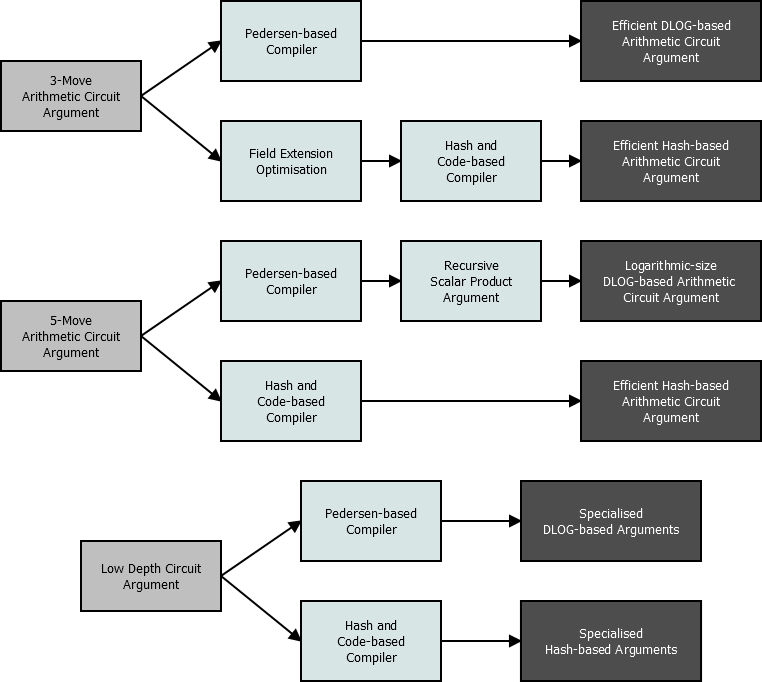
\includegraphics{recipes.png}
}
\caption{Different ways to combine the results in this thesis.}\label{fig:recipes}
\end{figure}